\thispagestyle{formato-PI}
\renewcommand{\MayorVer}{2}
\renewcommand{\MenorVer}{0}
\renewcommand{\Titulo}{Verificación de termómetros}
\renewcommand{\TipoID}{PRO}
\renewcommand{\FechaPub}{2023--01}

\section{\Titulo}\index{Programa!metrología, de}\index{Procedimiento!verificación de termómetros}
\renewcommand{\Codigo}{\Prog--\thesection--\TipoID}

\subsection{Objetivo}

Mantener el equipo de medición de temperatura, para asegurar se realicen lecturas de temperaturas precisas y confiables.

\subsection{Alcance}

Todos los Termómetros de Red de Fríos.

\subsection{Terminología y definiciones}

\begin{itemize}
	\item \textbf{Verificación y Ajuste:} La verificación de los termómetros se lleva a cabo realizando comparativos de temperatura utilizando un termómetro patrón como referencia. Existe un formato F-OP-22 en el cual se llevan a cabo las verificaciones de los termómetros, si existiera alguna desviación de temperatura se dará ajuste al termómetro y será registrado %TODO
\end{itemize}

\subsection{Procedimiento}

\begin{enumerate}
	\item Llene un vaso de espuma plástica aislante con hielo.
	\item Agregue hielo, de preferencia molido.
	\item Agregue agua hasta llenar el vaso.
	\item Coloque la sonda del termómetro patrón en el vaso y revuelva continuamente hasta que el termómetro llegue a la temperatura de \qty{0}{\degreeCelsius}.
	\item Coloque el termómetro de aguja dentro del vaso asegurándose que registre la misma temperatura del termómetro patrón.
	\item Para verificar un termómetro infrarrojo de manera correcta, el termómetro deberá tener una inclinación de \ang{45} y una distancia de no más de \qty{5}{\centi\meter} del agua helada.
	\item Anote la temperatura o desviación en el formato de verificación y ajuste de termómetros.
	\item{\textbf{Nota 1:}} ver \cref{fig:IceBath} para el correcto procedimiento de hacer un baño de hielo.
    \item{\textbf{Nota 2:}} Verificar las instrucciones específicas de cada termómetro para realizar la calibración pertinente.
\end{enumerate}

\subsection{Responsables de la actividad}
\begin{itemize}
	\item \textbf{Ejecutado} por personal de aseguramiento de calidad.
\end{itemize}

\subsection{Acciones correctivas}
\subsubsection{Ajuste TRIM}
\begin{itemize}
	\item Si existe alguna diferencia de más de \qtyrange{+-0.5}{+-1}{\degreeCelsius} en la temperatura, el tornillo de metal situado en la base debajo de la escala deberá girarse hasta \qty{0}{\degreeCelsius} mientras el termómetro permanezca en el agua, no realizando más de 3 ajustes en la vida útil del termómetro.
	\item Remplazar termómetro.
\end{itemize}

\subsection{Frecuencia}

\begin{itemize}
	\item Verificación semanal;
	\item Calibración anual.
\end{itemize}

\begin{changelog}[title=Registro de cambios,simple, sectioncmd=\subsection*,label=changelog-\thesection-\MayorVer.\MenorVer]
	\begin{version}[v=\MayorVer.\MenorVer, date=2023--01, author=Pablo E. Alanis]
		\item Cambio de formato;
		\item Cambios en la serialización de versiones;
		\item Correcciones ortográficas y de estilo.
	\end{version}

	\begin{version}[v=1.7, date=2022--05, author=Alonso M.]
		\item cambio de fecha;
	\end{version}

	\shortversion{v=1.6, date=2021--05, changes=No hubo cambios}
\end{changelog}


\begin{figure}[p]
    \centering
    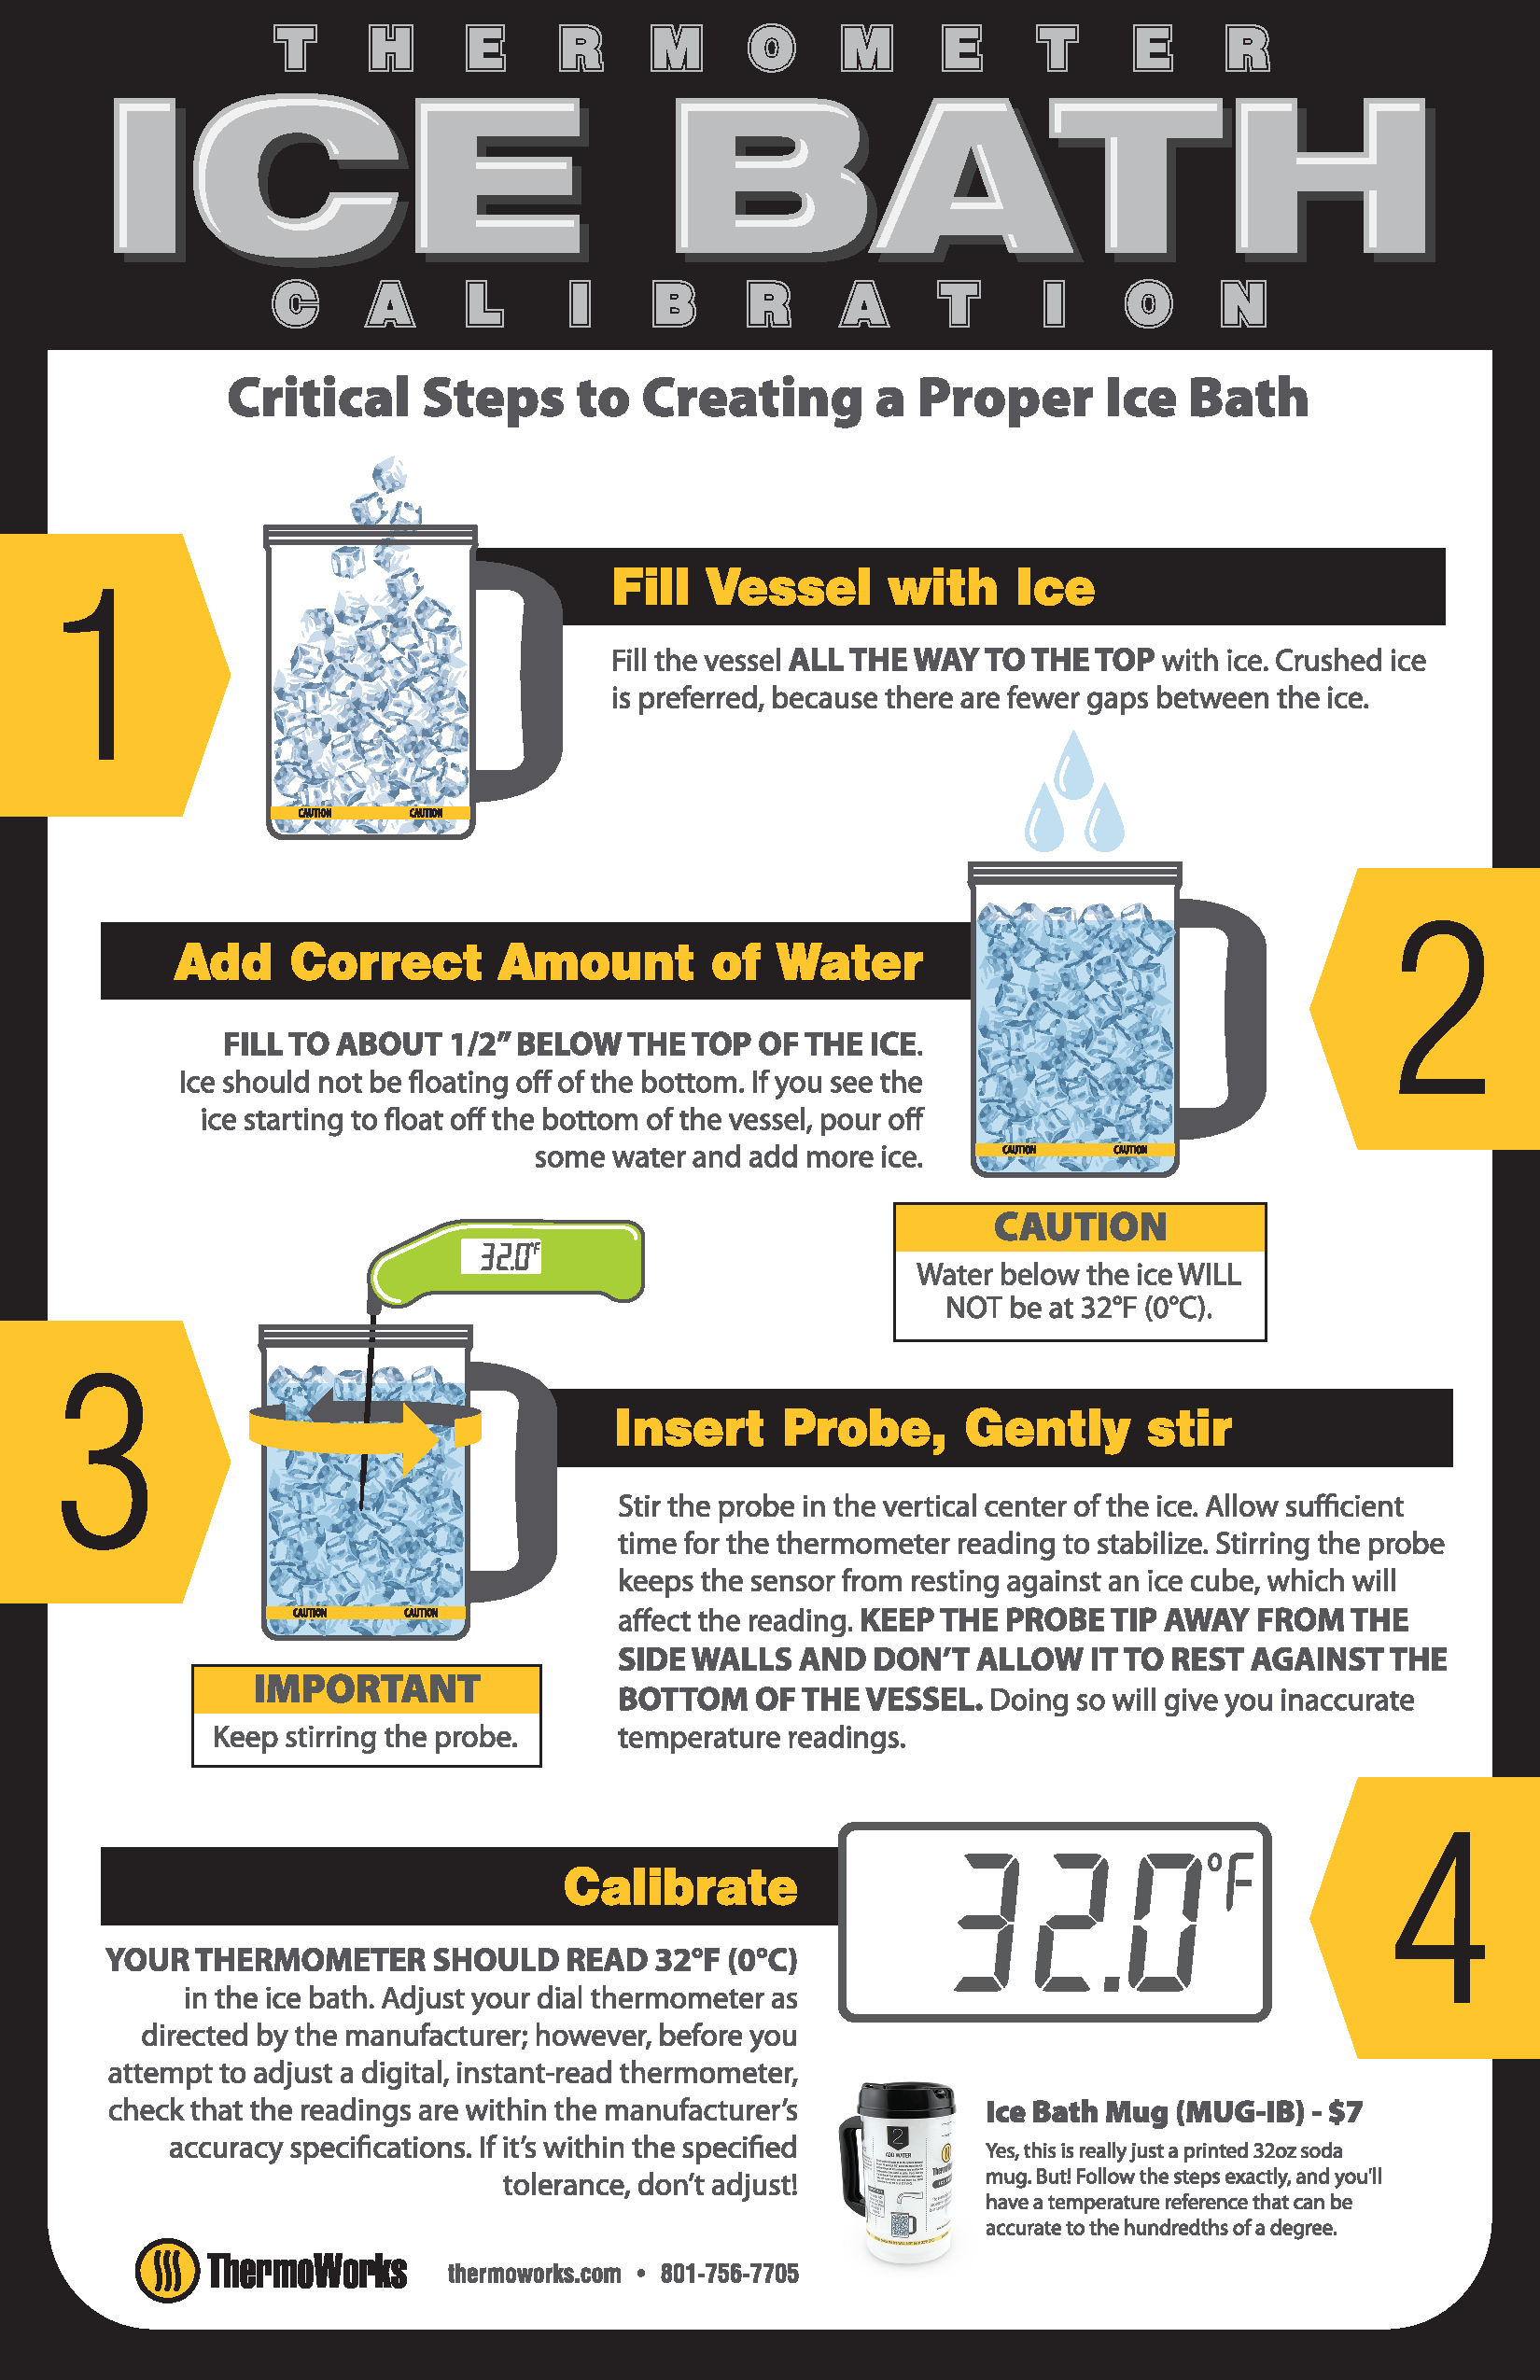
\includegraphics[height=0.85\textheight]{ref/ice_bath_infographic.pdf}
    \caption[Forma correcta de hacer un baño de hielo]{Forma correcta de hacer un baño de hielo}
    \label{fig:IceBath}
\end{figure}